% chktex-file 1
% !TeX spellcheck = en_GB
% !TeX program = pdflatex
%
% LuxSleek-CV 1.1 LaTeX template
% Author: Andreï V. Kostyrka, University of Luxembourg
%
% 1.1: added tracking and letter-spacing for prettier lower caps, added `~` for language levels
% 1.0: initial release
%
% This template fills the gap in the available variety of templates
% by proposing something that is not a custom class, not using any
% hard-coded settings deeply hidden in style files, and provides
% a handful of custom command definitions that are as transparent as it gets.
% Developed at the University of Luxembourg.
%
% *NOTHING IS HARCODED, and never should be.*
%
% Target audience: applicants in the IT industry, or business in general
%
% The main strength of this template is, it explicitly showcases how
% to break the flow of text to achieve the most flexible right alignment
% of dates for multiple configurations.

\documentclass[11pt, a4paper]{article}

\usepackage[T1]{fontenc}     % We are using pdfLaTeX,
\usepackage[utf8]{inputenc}  % hence this preparation
\usepackage[british]{babel}
\usepackage[left = 0mm, right = 0mm, top = 0mm, bottom = 0mm]{geometry}
\usepackage[stretch = 25, shrink = 25, tracking=true, letterspace=30]{microtype}
\usepackage{graphicx}        % To insert pictures
\usepackage{xcolor}          % To add colour to the document
\usepackage{marvosym}        % Provides icons for the contact details
\usepackage{fontawesome}

\usepackage{enumitem}        % To redefine spacing in lists
\setlist{parsep = 0pt, topsep = 0pt, partopsep = 1pt, itemsep = 1pt, leftmargin = 6mm}

\usepackage{FiraSans}        % Change this to use any font, but keep it simple
\renewcommand{\familydefault}{\sfdefault}

\definecolor{cvblue}{HTML}{304263}

%%%%%%% USER COMMAND DEFINITIONS %%%%%%%%%%%%%%%%%%%%%%%%%%%
% These are the real workhorses of this template
\newcommand{\dates}[1]{\hfill\mbox{\textbf{#1}}} % Bold stuff that doesn’t got broken into lines
\newcommand{\is}{\par\vskip.5ex plus .4ex} % Item spacing
\newcommand{\headleft}[1]{\vspace*{3ex}\textsc{\textbf{#1}}\par%
    \vspace*{-1.5ex}\hrulefill\par\vspace*{0.7ex}}
\newcommand{\headright}[1]{\vspace*{2.5ex}\textsc{\Large\color{cvblue}#1}\par%
     \vspace*{-2ex}{\color{cvblue}\hrulefill}\par}
\newcommand{\jobtitle}[2]{%
     \vspace{2ex} % add vertical space between entries if needed
     \textbf{\large #1} \\ % explicitly set the font size (e.g., \large)
     \hfill \textbf{\large #2} \\
   }
%%%%%%%%%%%%%%%%%%%%%%%%%%%%%%%%%%%%%%%%%%%%%%%%%%%%%%%%%%%%

\usepackage[colorlinks = true, urlcolor = white, linkcolor = white]{hyperref}

\begin{document}

% Style definitions -- killing the unnecessary space and adding the skips explicitly
\setlength{\topskip}{0pt}
\setlength{\parindent}{0pt}
\setlength{\parskip}{0pt}
\setlength{\fboxsep}{0pt}
\pagestyle{empty}
\raggedbottom

\begin{minipage}[t]{0.28\textwidth} %% Left column -- outer definition
%  Left column -- top dark rectangle
\colorbox{cvblue}{\begin{minipage}[t][5mm][t]{\textwidth}\null\hfill\null\end{minipage}}

\vspace{-.2ex} % Eliminates the small gap
\colorbox{cvblue!90}{\color{white}  %% LEFT BOX
\kern0.09\textwidth\relax% Left margin provided explicitly
\begin{minipage}[t][293mm][t]{0.82\textwidth}
\raggedright
\vspace*{2.5ex}

\Large Alex \textbf{\textsc{Jammes}} \normalsize

% Centering without extra vertical spacing
\null\hfill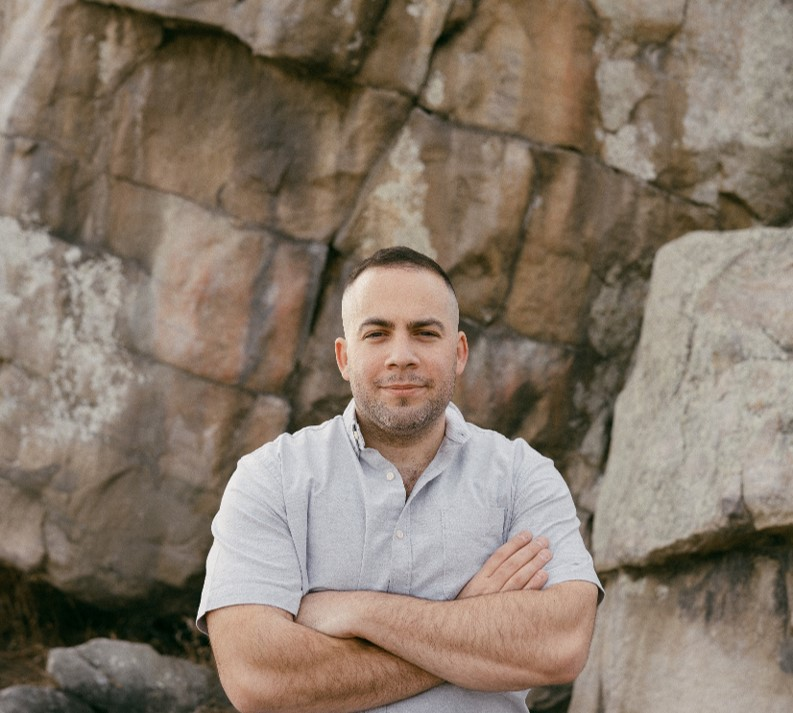
\includegraphics[width=0.65\textwidth]{images/resume_profile_picture.jpg}\hfill\null

\vspace*{0.5ex} % Extra space after the picture

\headleft{Profile Summary}
Dynamic and results-driven Cloud Architect with 8+ years of experience in \textit{technical solutions sales}, specializing in Public Cloud. Proven success in exceeding targets and fostering strong relationships, particularly within Federal and Enterprise sectors. Skilled in guiding customers through the full sales cycle, enabling strategic cloud adoption, and driving significant growth while building enduring partnerships.

\headleft{Contact details}
\small % To fit more content
\MVAt\ {\small ajammes.ftnt@gmail.com} \\[0.4ex]
\faGithub\ {\small github.com/AJLab-GH}\\[0.2ex]
\Mobilefone\ +1\,613\,889\,6564\,\\

\normalsize

\headleft{Personal information}
Citizenship: \textbf{Canadian} \\[0.5ex]
Clearance: \textbf{Secret (2026), Top-Secret Elligibility} \\[0.5ex]
Languages: \textbf{English}, \textbf{French}

\headleft{Skills}
\begin{itemize}
\item Azure, Amazon Web Services, Google Cloud Platform, Oracle Cloud Infrastructure
\item Terraform, AWS CloudFormation, Azure Resource Manager (JSON, BICEP)
\item Docker, Kubernetes, AKS, EKS
\item Azure Pipelines, AWS Code Pipeline, Azure DevOps, Jenkins
\item CPSM, CWPP, CIEM, CNAPP
\end{itemize}

\end{minipage}%
\kern0.09\textwidth\relax%%Right margin provided explicitly to stretch the colourbox
}
\end{minipage}% Right column
\hskip2.5em% Left margin for the white area
\begin{minipage}[t]{0.61\textwidth}
\setlength{\parskip}{0.8ex}% Adds spaces between paragraphs; use \\ to add new lines without this space. Shrink this amount to fit more data vertically

\vspace{2ex}

\headright{Experience}

\vspace{-4mm}
\jobtitle{Consulting System Engineer --- Cloud Architect at Fortinet (Canada)}{2022.04--Present}

\textbf{\small{Strategic Sales \& Technical Support:}} \small{Acted as a key technical resource for strategic pre-sales engagements across Canada. Designed tailored security solutions, driving customer success and satisfaction.}

\is
\textbf{\small{Customer \& Partner Engagement:}} \small{Led high-impact technical meetings, presentations, and product demonstrations, highlighting Fortinet’s strengths and value. Spearheaded webinars, conference talks, and events, including co-presentations with Microsoft at Azure Public Sector events and collaboration with AWS around their LZA solution. Engaged with partners and customers through various platforms to drive cloud adoption and showcase technical leadership.}

\is
\textbf{\small{Cloud Architecture \& Security:}} \small{Architected secure cloud networks in competitive scenarios, leveraging Fortinet’s product line. Led integrations with AWS Secure Environment Accelerator, AWS Landing Zone Accelerator, Microsoft Azure's Cloud Adoption Framework: Enterprise Scale Architecture (including CanPubSecALZ), and GCP and OCI's Public Sector Landing Zones.}

\is
\textbf{\small{Technical Consultancy \& Cross-Functional Collaboration:}} \small{Served as a subject-matter expert in pre-sales design reviews and collaborated with product management to identify, qualify, and develop key features. Enabled Business Development Engineers and Field Engineering to align with industry trends by providing them with the necessary tooling, insights, and guidance, ensuring strategic alignment and effective customer engagements.}

\is
\textbf{\small{Executive Engagement:}} \small{Engaged with executives and key decision-makers, participating in EBCs to articulate high-impact cloud strategies and solutions. Leveraged business drivers and industry insights to present complex cloud concepts in a clear and actionable manner, facilitating strategic alignment and driving cloud adoption at the executive level.}

\jobtitle{Presales Security Expert --- Cloud Architect at Fortinet (Federal)}{2019.06--2022.04}

\is
\textbf{\small{Strategic Cloud Partnerships:}} \small{Established key partnerships with cloud service providers, collaboratively selling, deploying, and delivering integrated solutions that expedited the Security Assessment \& Authorization (SA\&A) process, enabling customers to quickly attain their Authority to Operate (ATO) and achieve operational readiness in the cloud.}

\is
\textbf{\small{Federal Sector Selling:}} \small{Successfully sold tailored solutions to the Federal vertical, enhancing company presence in the sector.}

\is
\textbf{\small{High-Value Deals:}} \small{Closed multiple significant deals, driving substantial revenue growth.}

\jobtitle{Diamond Services Engineer \& TAC at Check Point (North-America)}{2017.01--2019.06}

\textbf{\small{Customer Engagement:}} \small{Played a key role in the design, deployment, and maintenance of cloud security solutions for Fortune 100 companies. Additionally, led training on public and private cloud solutions for both internal stakeholders and customers across Canada, the United States, and internationally.}

\headright{Education}

\textsc{Network Security Professional Program.} \textit{from Willis College}. \dates{2015--2016} \\

\headright{Fun Facts}

\textit{This resume was created and delivered as Code.}

\end{minipage}

\end{document}
